%Adaptado de
%=========
%% bare_jrnl.tex
%% V1.4b
%% 2015/08/26
%% by Michael Shell
%=======
%Definición del tipo de documento
\documentclass[journal]{IEEEtran}
%Paquetes que se usarán
%Paquete de codificación
\usepackage[utf8]{inputenc}
%Paquete de idioma
\usepackage[spanish]{babel}
%Paquete para manejo de URLs.
\usepackage{hyperref}
%Paquete para manejo general de imágenes
\usepackage{graphicx}
%También se puede(n) indicar la ubicación de algunas carpetas que contienen diversos documentos, imágenes, código, bibliografía, etc.
%\addbibresource{mybibliography.bib}
\graphicspath{{./Imagenes/}}

\begin{document}
\title{Plantilla para presentación de trabajos en\\ Ingeniería de Sistemas UniMinuto 2019}

\author{Michael~Shell,~\IEEEmembership{Member,~IEEE,}
        John~Doe,~\IEEEmembership{Fellow,~OSA,}
        and~Jane~Doe,~\IEEEmembership{Life~Fellow,~IEEE}% <-this % stops a space
\thanks{M. Shell was with the Department
of Electrical and Computer Engineering, Georgia Institute of Technology, Atlanta,
GA, 30332 USA e-mail: (see http://www.michaelshell.org/contact.html).}% <-this % stops a space
\thanks{J. Doe and J. Doe are with Anonymous University.}% <-this % stops a space
\thanks{Manuscript received April 19, 2005; revised August 26, 2015.}}

% The paper headers
\markboth{Asignatura correspondiente - Año - Semestre}{}

% make the title area
\maketitle

\begin{abstract}
El resumen viene acá. Se recomiendan máximo 200 palabras, o máximo 800 caracteres (contando espacios). No introducir fórmulas, símbolos o similares.
\end{abstract}

% Note that keywords are not normally used for peerreview papers.
\begin{IEEEkeywords}
Palabra clave 1, palabra clave 2, etc.
\end{IEEEkeywords}

\section{Introducción}

\IEEEPARstart{E}{sta} plantilla permite a los estudiantes de ingeniería de sistemas, de las asignaturas [Aquí van las asignaturas] poder presentar sus trabajos parciales y de fin de curso, de acuerdo a las especificaciones impartidas en clase.\\
% You must have at least 2 lines in the paragraph with the drop letter
% (should never be an issue)
"Si algo puede ir mal, saldrá mal y de la peor forma, siempre".
Pueden insertarse símbolos especiales. Leer la documentación en:  \url{https://www.overleaf.com/learn/latex/Main_Page}.

\subsection{A veces hay subsecciones}
También se pueden colocar los hipervínculos de forma tal que "no se vean", sino se haga un llamado dentro del texto, así:\\
\href{https://www.overleaf.com/learn/latex/Main_Page}{Documentación de LaTex}.\par
Se recomienda usar un \emph{urlShortener} para evitar símbolos extraños al compilador o longitud excesiva y poco fácil de manejar.

\subsubsection{Y pueden haber sub-subsecciones}
Se pueden generar viñetas:
\begin{itemize}
    \item Alguno
    \item Otro
\end{itemize}
O se pueden numerar:
\begin{enumerate}
    \item Uno
    \item Dos
\end{enumerate}
Y se pueden indentar unos dentro de otros:
\begin{enumerate}
    \item Uno
    \begin{enumerate}
        \item Uno.a
        \item Uno.b
    \end{enumerate}
    \item Dos
    \begin{itemize}
        \item Dos algo
        \item Dos otro
    \end{itemize}
\end{enumerate}
\section{Segunda parte}
Se pueden insertar gráficos y también se  pueden insertar imágenes con numeración (y centradas). Ejemplo: Véase la figura \ref{fig:calvin1}.
\begin{figure}
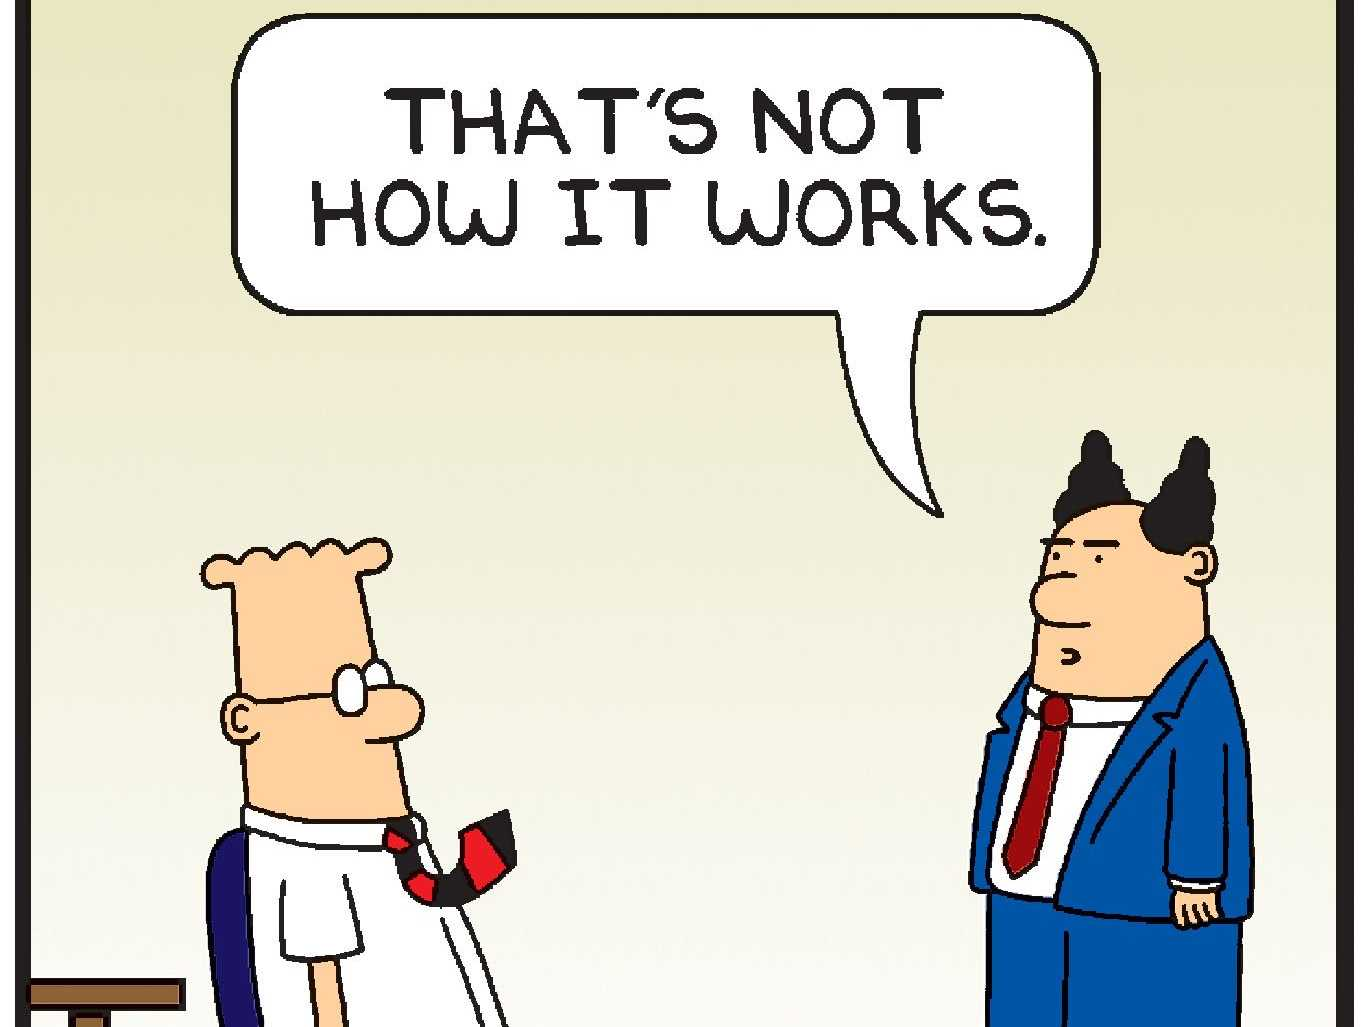
\includegraphics[scale = 0.1]{Imagenes/Dilbert.jpg}
\end{figure}

\begin{figure}
\caption{Si el \emph{caption} va antes}
%\centering

\includegraphics[width=0.4\textwidth]{Imagenes/CandH1.jpg}
\label{fig:calvin1}
\end{figure}

\begin{figure}[h!]
\centering

\includegraphics[width=0.25\textwidth]{Imagenes/simon_circ.png}
\caption{Si el \emph{caption} va después}
\end{figure}

\section{Conclusiones}
¿Qué sucede con las tablas?\\
En la documentación se encuentra el código, explicado y con ejemplos, para esto.

% Si hay un solo apéndice:
\appendix[Título del apéndice]
Generalmente se maneja un único apéndice, con \emph{further explanation}. Procure evitar los términos en otros idiomas a no ser que sean técnicos o no traducibles.

%appendices
%\section{¿Para qué se usarán varios apéndices en un documento?}

%\section{¿Para qué se usarán otros apéndices en un documento?}

% you can choose not to have a title for an appendix
% if you want by leaving the argument blank


% use section* for acknowledgment
\section*{Agradecimientos}
En caso tal que sea conveniente o necesario: a mis patrocinadores, al profe que tuvo confianza en mi, a la afición tan bonita que nos acompaña, et.
% Can use something like this to put references on a page by themselves when using endfloat and the captionsoff option.
\ifCLASSOPTIONcaptionsoff
  \newpage
\fi

\begin{thebibliography}{1}

\bibitem{IEEEhowto:kopka}
H.~Kopka and P.~W. Daly, \emph{A Guide to \LaTeX}, 3rd~ed.\hskip 1em plus
  0.5em minus 0.4em\relax Harlow, England: Addison-Wesley, 1999.

\end{thebibliography}
\end{document}

